%%%%%%%%%%%%%% 02/03/2020 %%%%%%%%%%%%%%%% 
\subsection*{\textbf{02/03/2020}}

\subsubsection{Days Aim}
\begin{itemize}
    \item Continue to investigate potential cuts for Zee and Zmumu and calculate cross sections.
\end{itemize}
\subsubsection{Day Summary}
\begin{itemize}
    \item Made stacked log plots of invariant mass, transverse momentum and the isolation variables.
    \item Began investigation of Higgs decay to 4 leptons
\end{itemize}


%%%%%%%%%%%%% 08:40 %%%%%%%%%%%%%
\subsubsection*{08:40 - Lead BG - Plotting invariant mass plots using the cuts used to calculate $\sigma$ so far}

%%%%%%%%%%%%% 08:41 %%%%%%%%%%%%%
\subsubsection*{08:41 - Invariant mass plot of ee}
Cuts used in Fig.\ref{fig:08-41_02-02-21}

\begin{lstlisting}
basic_cut = "(lep_charge[0] != lep_charge[1]) && (lep_type[0] == 11 && lep_type[1] == 11) && lep_n==2"

inv_mass_cut = "(inv_mass_Zll > 70e3) && (inv_mass_Zll < 150e3)"

etcone_cut = "(lep_etcone20[0] > -2e3 && lep_etcone20[1] > -2e3)" + "&& (lep_etcone20[0] < 6e3 && lep_etcone20[1] < 6e3)"

ptcone_cut = "(lep_ptcone30[0] < 5.8e3) && (lep_ptcone30[1] < 5.8e3)"

pt_cut = "(lep_pt[0] > 35e3) && (lep_pt[1] > 35e3)"
    
lepCut = "(" + basic_cut + "&&" + inv_mass_cut + "&&" + etcone_cut + "&&" + ptcone_cut + "&&" + pt_cut + ")"
    
t.SetAlias("inv_mass_Zll","sqrt(2*lep_pt[0]*lep_pt[1]*(cosh(lep_eta[0]-lep_eta[1])-cos(lep_phi[0]-lep_phi[1])))")
  
t.Draw("inv_mass_Zll >> h_inv_mass_Zll(100,0e3,200e3)", weighting + "*" + lepCut)
\end{lstlisting}

\begin{figure}[h!]
    \centering
    \begin{minipage}{0.5\textwidth}
        \centering
        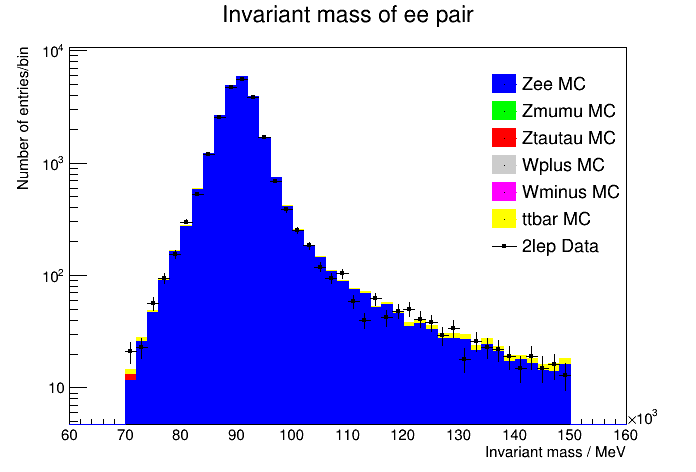
\includegraphics[width=\linewidth]{plots/02-03-2021/08-41_invar-mass.png}
        (A)
    \end{minipage}\hfill
    \begin{minipage}{0.5\textwidth}
        \centering
        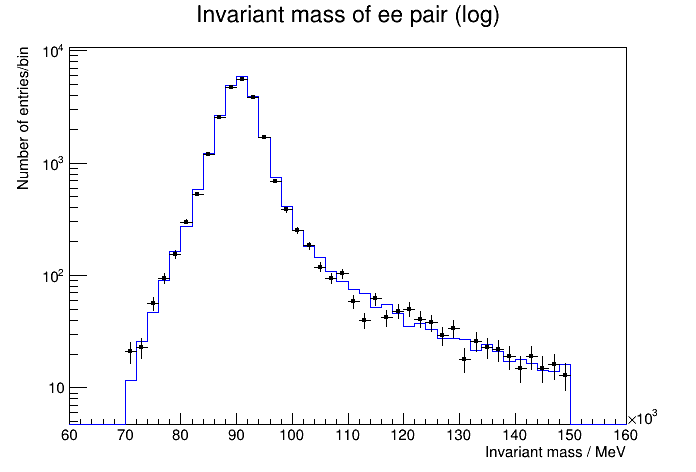
\includegraphics[width=\linewidth]{plots/02-03-2021/08-46_2-Stack_2lep_Zee_invar-mass.png}
        (B)
    \end{minipage}
    \caption{(A) Invariant mass of pair of electrons using ATLAS, Zee MC, and background MC.  (B)Invariant mass of pair of electrons using ATLAS and Zee MC.  Cuts: basic plus all others\dots}
    \label{fig:08-41_02-02-21}
\end{figure}

%%%%%%%%%%%%% 08:58 %%%%%%%%%%%%%
\subsubsection*{08:58 - Invariant mass ee basic}
Cuts used in Fig.\ref{fig:08-58_02-03-21}:
\begin{lstlisting}
 basic_cut = "(lep_charge[0] != lep_charge[1]) && (lep_type[0] == 11 && lep_type[1] == 11) && lep_n==2"

lepCut = "(" + basic_cut + ")"

    
t.SetAlias("inv_mass_Zll","sqrt(2*lep_pt[0]*lep_pt[1]*(cosh(lep_eta[0]-lep_eta[1])-cos(lep_phi[0]-lep_phi[1])))")
  
t.Draw("inv_mass_Zll >> h_inv_mass_Zll(100,0e3,200e3)", weighting + "*" + lepCut)
\end{lstlisting}

\begin{figure}[h!]
    \centering
    \begin{minipage}{0.5\textwidth}
        \centering
        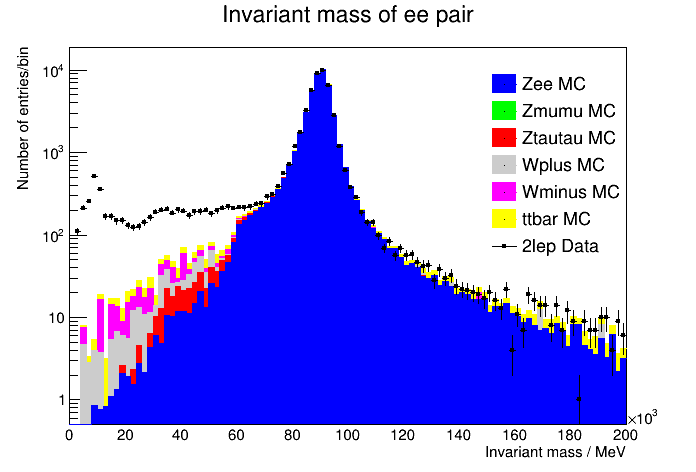
\includegraphics[width=\linewidth]{plots/02-03-2021/08-58_basic.png}
        (A)
    \end{minipage}\hfill
    \begin{minipage}{0.5\textwidth}
        \centering
        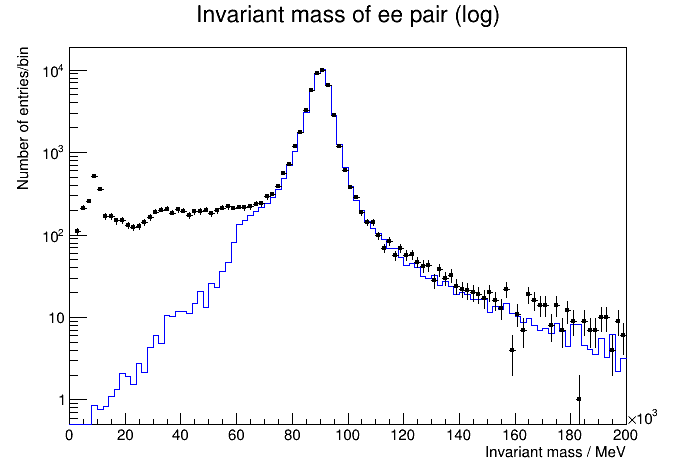
\includegraphics[width=\linewidth]{plots/02-03-2021/08-59_2Stack.png}
        (B)
    \end{minipage}
    \caption{(A) Invariant mass of pair of electrons using ATLAS, Zee MC, and background MC.  (B)Invariant mass of pair of electrons using ATLAS and Zee MC.  Cuts: basic only}
    \label{fig:08-58_02-03-21}
\end{figure}

%%%%%%%%%%%%% 09:24 %%%%%%%%%%%%%
\subsubsection*{09:24 - Invariant mass ee $-2 GeV < etcone < 6 GeV $}
Cuts used in Fig.\ref{fig:09:24_02-03-21}
\begin{lstlisting}
 basic_cut = "(lep_charge[0] != lep_charge[1]) && (lep_type[0] == 11 && lep_type[1] == 11) && lep_n==2"
 
 lepCut = "(" + basic_cut + "&&" + etcone_cut + ")"

 t.SetAlias("inv_mass_Zll","sqrt(2*lep_pt[0]*lep_pt[1]*(cosh(lep_eta[0]-lep_eta[1])-cos(lep_phi[0]-lep_phi[1])))")
  
 t.Draw("inv_mass_Zll >> h_inv_mass_Zll(100,0e3,200e3)", weighting + "*" + lepCut)
\end{lstlisting}


\begin{figure}[h!]
    \centering
    \begin{minipage}{0.5\textwidth}
        \centering
        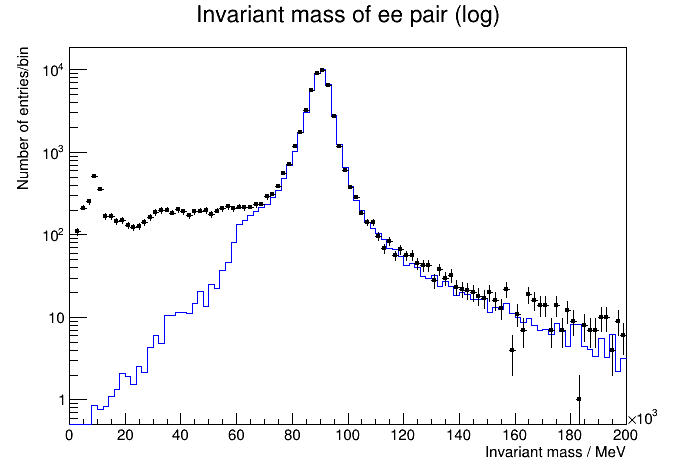
\includegraphics[width=\linewidth]{plots/02-03-2021/09-28_AllStack.png}
        (A)
    \end{minipage}\hfill
    \begin{minipage}{0.5\textwidth}
        \centering
        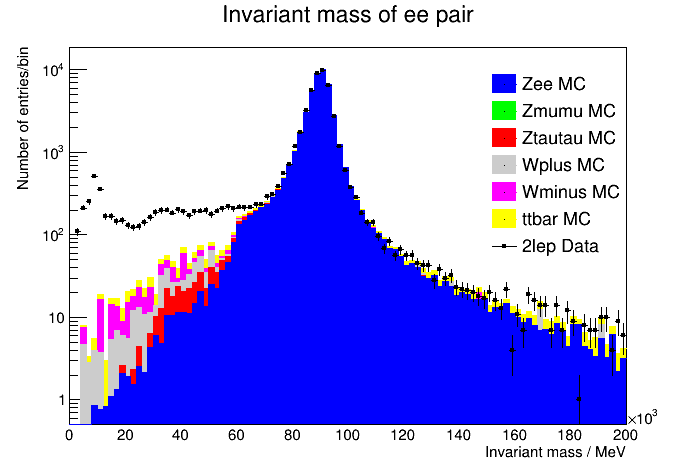
\includegraphics[width=\linewidth]{plots/02-03-2021/09-24_2Stack.png}
        (B)
    \end{minipage}
    \caption{(A)  (B). Cuts: basic plus upper and lower bound on etcone.}
    \label{fig:09:24_02-03-21}
\end{figure}


%%%%%%%%%%%%% 09:35 %%%%%%%%%%%%%
\subsubsection*{09:35 - Invariant mass ee $ptcone < 5.8 GeV $}
Cuts used in Fig.\ref{fig:09:35_02-03-21}
\begin{lstlisting}
basic_cut = "(lep_charge[0] != lep_charge[1]) && (lep_type[0] == 11 && lep_type[1] == 11) && lep_n==2"

ptcone_cut = "(lep_ptcone30[0] < 5.8e3) && (lep_ptcone30[1] < 5.8e3)"

lepCut = "(" + basic_cut + "&&" + ptcone_cut + ")"

t.SetAlias("inv_mass_Zll","sqrt(2*lep_pt[0]*lep_pt[1]*(cosh(lep_eta[0]-lep_eta[1])-cos(lep_phi[0]-lep_phi[1])))")
  
t.Draw("inv_mass_Zll >> h_inv_mass_Zll(100,0e3,200e3)", weighting + "*" + lepCut)
\end{lstlisting}
\begin{figure}[h!]
    \centering
    \begin{minipage}{0.5\textwidth}
        \centering
        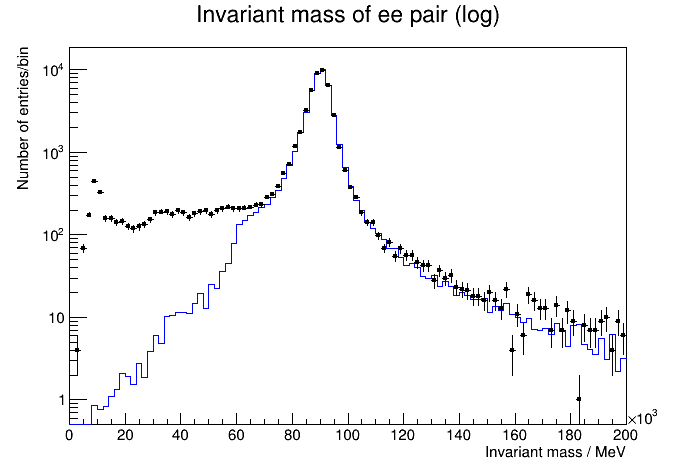
\includegraphics[width=\linewidth]{plots/02-03-2021/09-35_2Stack.png}
        (A)
    \end{minipage}\hfill
    \begin{minipage}{0.5\textwidth}
        \centering
        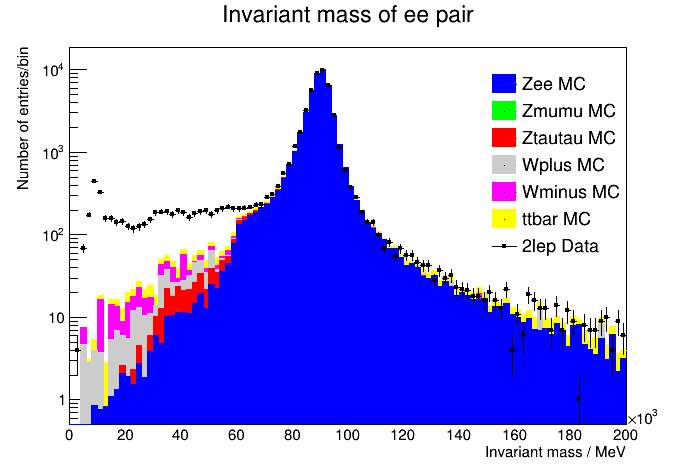
\includegraphics[width=\linewidth]{plots/02-03-2021/09-37_AllStack.png}
        (B)
    \end{minipage}
    \caption{(A)  (B) . Cuts: basic plus upper bound on ptcone = 5.8 GeV. $ptcone < 5.8 GeV$}
    \label{fig:09:35_02-03-21}
\end{figure}


%%%%%%%%%%%%% 09:45 %%%%%%%%%%%%%
\subsubsection*{09:45 - Invariant mass ee $pt > 35 GeV $}
Cuts used in Fig.\ref{fig:09:45_02-03-21}
\begin{lstlisting}
basic_cut = "(lep_charge[0] != lep_charge[1]) && (lep_type[0] == 11 && lep_type[1] == 11) && lep_n==2"

pt_cut = "(lep_pt[0] > 35e3) && (lep_pt[1] > 35e3)"
    
lepCut = "(" + basic_cut + "&&" + pt_cut + ")"
\end{lstlisting}
\begin{figure}[h!]
    \centering
    \begin{minipage}{0.5\textwidth}
        \centering
        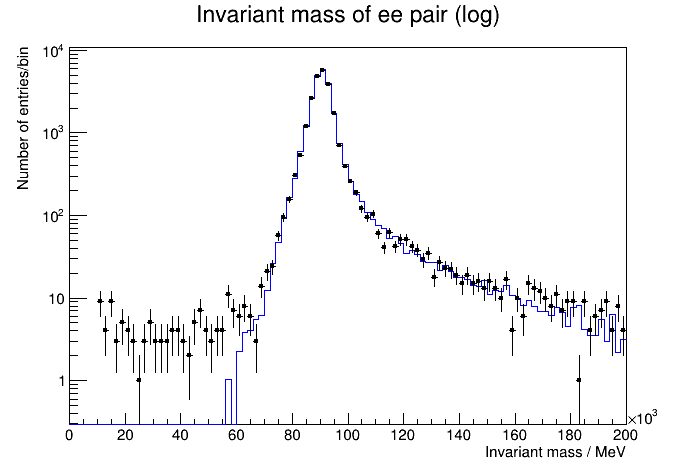
\includegraphics[width=\linewidth]{plots/02-03-2021/09-46_2Stack.png}
        (A)
    \end{minipage}\hfill
    \begin{minipage}{0.5\textwidth}
        \centering
        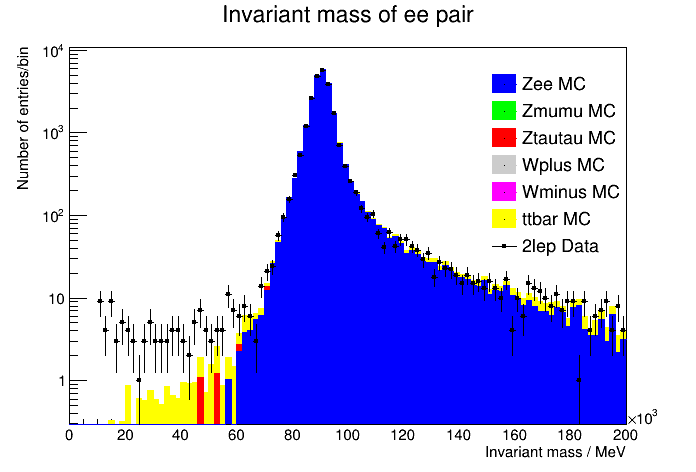
\includegraphics[width=\linewidth]{plots/02-03-2021/09-45_AllStack.png}
        (B)
    \end{minipage}
    \caption{(A)  (B). Basic cuts plus $pt > 35 GeV $}
    \label{fig:09:45_02-03-21}
\end{figure}

%%%%%%%%%%%%% 10:23 %%%%%%%%%%%%%
\subsubsection*{10:23 - Invariant mass ee etcone, ptcone and pt cuts}
Cuts used in Fig.\ref{fig:10:10_02-03-21}
\begin{lstlisting}
basic_cut = "(lep_charge[0] != lep_charge[1]) && (lep_type[0] == 11 && lep_type[1] == 11) && lep_n==2"

etcone_cut = "(lep_etcone20[0] > -2e3 && lep_etcone20[1] > -2e3)" + "&& (lep_etcone20[0] < 6e3 && lep_etcone20[1] < 6e3)"

ptcone_cut = "(lep_ptcone30[0] < 5.8e3) && (lep_ptcone30[1] < 5.8e3)"

pt_cut = "(lep_pt[0] > 35e3) && (lep_pt[1] > 35e3)"

lepCut = "(" + basic_cut + "&&" + etcone_cut + "&&" + ptcone_cut + "&&" + pt_cut + ")"
\end{lstlisting}
\begin{figure}[h!]
    \centering
    \begin{minipage}{0.5\textwidth}
        \centering
        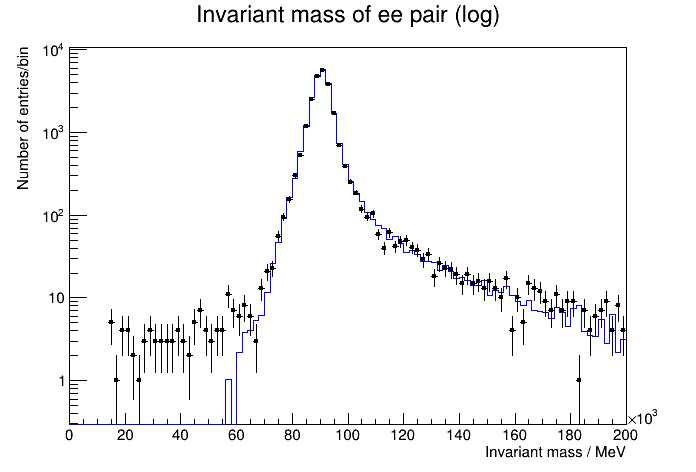
\includegraphics[width=\linewidth]{plots/02-03-2021/10-23_2Stack.png}
        (A)
    \end{minipage}\hfill
    \begin{minipage}{0.5\textwidth}
        \centering
        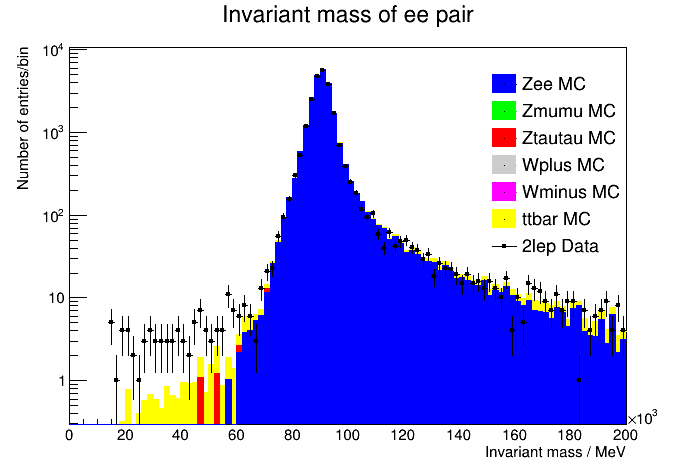
\includegraphics[width=\linewidth]{plots/02-03-2021/10-27_AllStack.png}
        (B)
    \end{minipage}
    \caption{(A)  (B). Basic cuts plus $pt > 35 GeV $, $ptcone < 5.8 GeV$, $-2 GeV < etcone < 6 GeV $}
    \label{fig:10:10_02-03-21}
\end{figure}


%%%%%%%%%%%%% 10:35 %%%%%%%%%%%%%
\subsubsection*{10:35 - ptcone ee (single e). Cuts: $pt > 35 GeV$}
Cuts used in Fig.\ref{fig:10:10_35-03-21}
\begin{lstlisting}
basic_cut = "(lep_charge[0] != lep_charge[1]) && (lep_type[0] == 11 && lep_type[1] == 11) && lep_n==2"

pt_cut = "(lep_pt[0] > 35e3) && (lep_pt[1] > 35e3)"
    
lepCut = "(" + basic_cut + "&&" + pt_cut + ")"
    
t.Draw("lep_ptcone30[0] >> h_lep_ptcone30(300,1e3,15e3)", weighting + "*" + lepCut)
\end{lstlisting}
\begin{figure}[h!]
    \centering
    \begin{minipage}{0.5\textwidth}
        \centering
        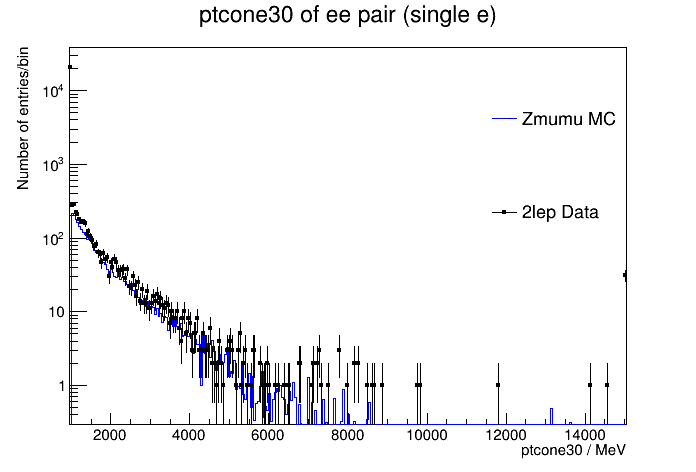
\includegraphics[width=\linewidth]{plots/02-03-2021/10-37_2Stack.png}
        (A)
    \end{minipage}\hfill
    \begin{minipage}{0.5\textwidth}
        \centering
        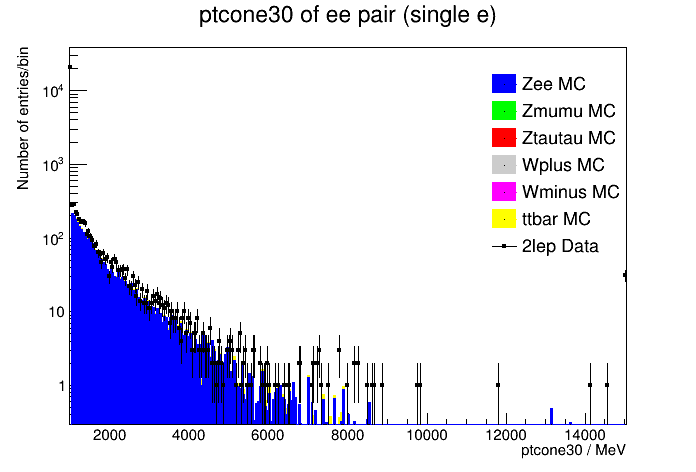
\includegraphics[width=\linewidth]{plots/02-03-2021/10-35_AllStack.png}
        (B)
    \end{minipage}
    \caption{(A) Ptcone30 of ATLAS and Zee MC data. (B) . Basic cuts plus $pt > 35 GeV$}
    \label{}
\end{figure}
Can therefore justify the upper bound on the ptcone30. of $ptcone < 5.8 GeV$


%%%%%%%%%%%%% 10:45 %%%%%%%%%%%%%
\subsubsection*{10:45 - etcone ee (single e). Cuts: $pt > 35 GeV$}
Cuts used in Fig.\ref{fig:10:10_45-03-21}
\begin{lstlisting}

\end{lstlisting}
\begin{figure}[h!]
    \centering
    \begin{minipage}{0.5\textwidth}
        \centering
        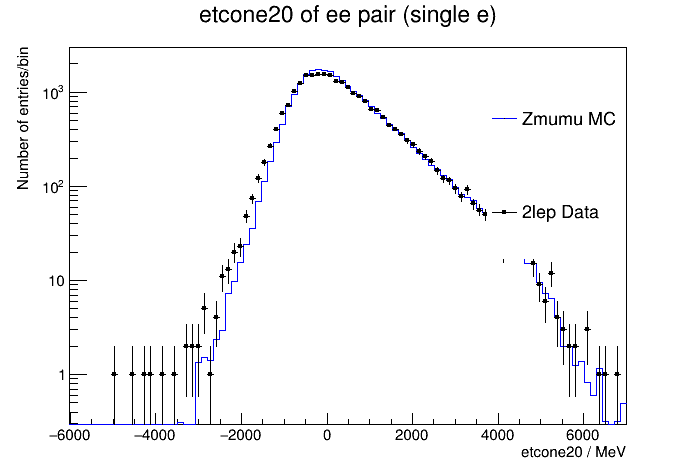
\includegraphics[width=\linewidth]{plots/02-03-2021/10-50_2Stack.png}
        (A)
    \end{minipage}\hfill
    \begin{minipage}{0.5\textwidth}
        \centering
        \includegraphics[width=\linewidth]{plots/02-03-2021/}
        (B)
    \end{minipage}
    \caption{(A)  (B)}
    \label{}
\end{figure}

%%%%%%%%%%%%% 15:20 %%%%%%%%%%%%%
\subsubsection*{15:20 - Invariant mass of 4lep for Higgs}


\textbf{Exercise 6.8:}\\
Verify expression for $m_{llll}$ for the decay $H \rightarrow \l^+ \l^- \l^+ \l^- $.
\begin{itemize}
    \item{Start by recalling the equation for the invarient mass of a system:}
    
\begin{align}
    m_{llll}^2 = E^2 - |\mathbf{p}|^2
\end{align}

\item{Now, working in index notation where $i,j = 1,2,3,4$ and $i\neq j$ (summing over $i$ and $j$), we can write:}

\begin{align}
     m_{llll}^2 = (E_i^2+ 2E_iE_j) -(|\mathbf{p_i}|^2+2\mathbf{p_i\cdot p_j}) \approx 2(|\mathbf{p_i|| p_j}|-\mathbf{p_i\cdot p_j})
\end{align}     
\item{Converting to kinematic variables as in excersise 6.2/3 gives us}

\begin{align}
    m_{llll}^2 = 2p_{Ti}p_{Tj}\left(\cosh{(\eta_i-\eta_i)}- \cos{(\phi_i - \phi_j)}\right)
\end{align}
\end{itemize}


Plot the invariant mass of 4 leptons using:
\begin{lstlisting}
    # Calulcate invariant mass of Higgs from the 4 leptons.
    x = "2 * lep_pt[{0}] * lep_pt[{1}]*(cosh(lep_eta[{0}]-lep_eta[{1}]) - cos(lep_phi[{0}]-lep_phi[{1}]))"
    s = ""

    for i in range(4):
        for j in range(i+1, 4):
            if not (i == 0 and j == 1):
                s += "+"
            s += x.format(i, j)
 
    t.SetAlias("s", s)
    t.SetAlias("inv_mass_4", "sqrt(s)")

    lepCut ="(" + "lep_n==4" + ")"
    
    t.Draw("inv_mass_4 >> h_inv_mass_4(80,0e3,500e3)", weighting + "*" + lepCut)
\end{lstlisting}
Cuts used in Fig.\ref{fig:15:20_02-03-21}:
\begin{lstlisting}
lepCut ="(" + "lep_n==4" + ")"
\end{lstlisting}

\begin{figure}[h!]
    \centering
	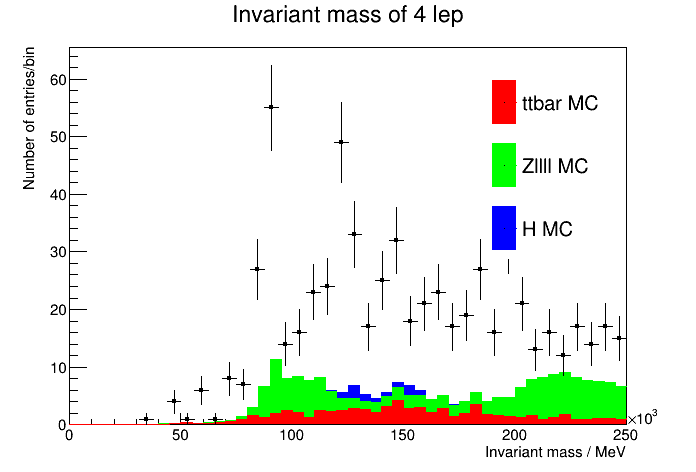
\includegraphics[width=0.85\linewidth]{plots/02-03-2021/15-20.png}
    \caption{Invariant mass plot using ATLAS and Higgs MC data.  Only basic cuts }
    \label{fig:15:20_02-03-21}
\end{figure}
    
%%%%%%%%%%%%% 17:00 %%%%%%%%%%%%%
\subsubsection*{17:00 - Invariant mass of 4lep for Higgs with only ee mumu, ee ee, mumu mumu}
Adding the cuts such that only allowed end products are allowed.
\\
Cuts used in Fig.\ref{fig:17:00_02-03-21}
\begin{lstlisting}
    # Allowed processes: ee mumu, ee ee, mumu mumu
    # For an allowed process, the sum of charge * type == 0 
    t_c_b = "(lep_charge[{0}] * lep_type[{0}])"  
    t_c = ""
    
    for i in range(4):
        if i != 0:
            t_c += " + "
        t_c += t_c_b.format(i)

    t.SetAlias("t_c_sum", t_c)
    t_c_cut = "t_c_sum == 0"
    
    ...
    
    lepCut ="(" + "lep_n==4" + "&&" + t_c_cut + ")"
    
    t.Draw("inv_mass_4 >> h_inv_mass_4(80,0e3,500e3)", weighting + "*" + lepCut)
\end{lstlisting}
\begin{figure}[h!]
    \centering
	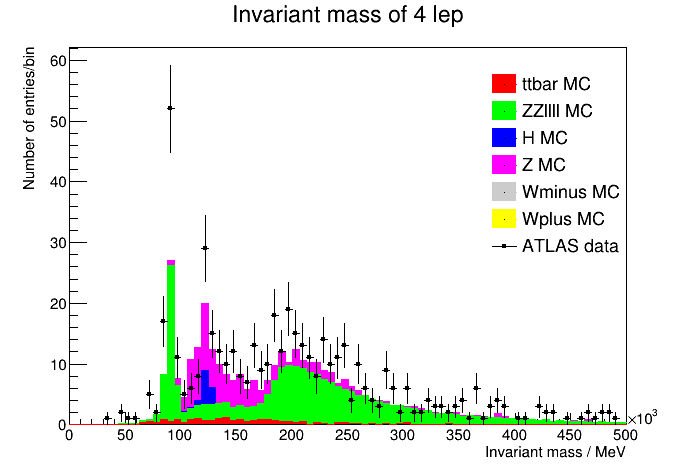
\includegraphics[width=0.85\linewidth]{plots/02-03-2021/17-00.png}
    \caption{Invariant mass plot using ATLAS and Higgs MC data.  Cuts: lep-n == 4, only allowed end products: == e+e- mu+mu-, e+e-e+e-, mu+mu- mu+mu-}
    \label{fig:17:00_02-03-21}
\end{figure}

%%%%%%%%%%%%% 17:30 %%%%%%%%%%%%%
\subsubsection*{17:30 - Investigate the invariant mass of lepton pairs (produced from 4 lepton producing events)}
Plot the invariant mass of lepton pair for lepton 0 and 1. = Fig.\ref{fig:17-30_02-03-21}.A
\\
Plot the invariant mass of lepton pair for lepton 2 and 3. = Fig.\ref{fig:17-30_02-03-21}.B
\\
Cuts used in Fig.\ref{fig:17-30_02-03-21}:
\begin{lstlisting}
    # Allowed processes: ee mumu, ee ee, mumu mumu
    # For an allowed process, the sum of charge * type == 0 
    t_c_b = "(lep_charge[{0}] * lep_type[{0}])"  
    t_c = ""
    
    for i in range(4):
        if i != 0:
            t_c += " + "
        t_c += t_c_b.format(i)

    t.SetAlias("t_c_sum", t_c)
    t_c_cut = "t_c_sum == 0"
    
    # Invariant mass of the two lepton pairs 
    # each have to be within the mass width of Z boson.
    # Will have mulitple pair cominations so need to calculate invariant mass for all possible combinations (combinatorics)
    lep2_invar_mass_str = "sqrt(2*lep_pt[{0}]*lep_pt[{1}]*(cosh(lep_eta[{0}]-lep_eta[{1}])-cos(lep_phi[{0}]-lep_phi[{1}])))"
    t.SetAlias("lep2_inv_mass", lep2_invar_mass_str.format(0, 1))
    
    lepCut ="(" + "lep_n==4" + "&&" + t_c_cut + ")"
    
    t.Draw("lep2_inv_mass >> lep2_inv_mass(80,0e3,500e3)", weighting + "*" + lepCut)
\end{lstlisting}
\begin{figure}[h!]
    \centering
    \begin{minipage}{0.5\textwidth}
        \centering
        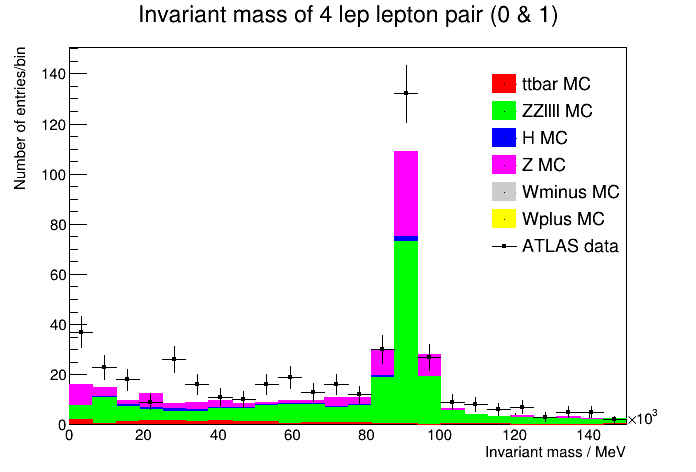
\includegraphics[width=\linewidth]{plots/02-03-2021/17-30_0-1.png}
        (A)
    \end{minipage}\hfill
    \begin{minipage}{0.5\textwidth}
        \centering
        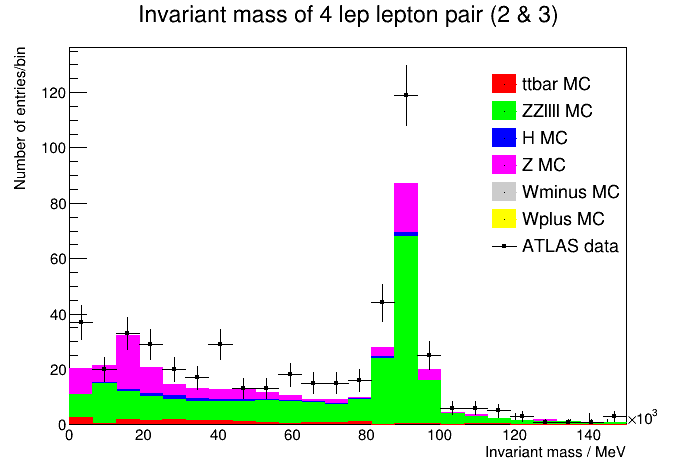
\includegraphics[width=\linewidth]{plots/02-03-2021/17-30_2-3.png}
        (B)
    \end{minipage}
    \caption{(A) Invariant mass of lepton pair using leptons 0 and 1. (B) Invariant mass of lepton pair using leptons 2 and 3.  Cuts used: lep-n==4,  allowed end products == e+e- mu+mu-, e+e-e+e-, mu+mu- mu+mu-}
    \label{fig:17-30_02-03-21}
\end{figure}

%%%%%%%%%%%%% 18:00 %%%%%%%%%%%%%
\subsubsection*{18:00 - Invariant mass of 4lep for Higgs with invariant mass cuts of lepton pairs}
Applying the cuts to provide bounds on the invariant mass of the possible combinations of the lepton pairs.
\\
With one Z boson being real, one pair of leptons should be the invariant mass range of $60 GeV < m_{ll} < 150 GeV$.
\\
With the other Z boson being virtual, the other pair of leptons should have an upper bound on the invariant mass of $m_{ll} < 150 GeV$.
\\
Cuts used in Fig.\ref{}:
\begin{lstlisting}
    # Allowed processes: ee mumu, ee ee, mumu mumu
    # For an allowed process, the sum of charge * type == 0 
    t_c_b = "(lep_charge[{0}] * lep_type[{0}])"  
    t_c = ""
    
    for i in range(4):
        if i != 0:
            t_c += " + "
        t_c += t_c_b.format(i)

    t.SetAlias("t_c_sum", t_c)
    t_c_cut = "t_c_sum == 0"
    
    # Invariant mass of the two lepton pairs 
    # one pair has to be within the mass width of Z boson.
    # with another which does not (the virtual z boson)
    # Will have mulitple pair cominations so need to calculate invariant mass for all possible combinations (combinatorics)

    lep2_invar_mass_str = "sqrt(2*lep_pt[{0}]*lep_pt[{1}]*(cosh(lep_eta[{0}]-lep_eta[{1}])-cos(lep_phi[{0}]-lep_phi[{1}])))"

    t_c_pair = "(lep_charge[{0}] * lep_type[{0}]) + (lep_charge[{1}] * lep_type[{1}])"

    lep_pair_inv_mass_cut = ""

    i = 0
    for j in range(1, 4):
        for k in range(1, 3):
            for l in range(2, 4):
                if j != k and j != l and k != l and k < l:
                    print(i,j,k,l)
                    if not (j == 1 and k == 2 and l == 3):
                        lep_pair_inv_mass_cut += " || "
                    lep_pair_inv_mass_cut += lep2_invar_mass_str.format(i, j) + " > 60e3 && " + lep2_invar_mass_str.format(i, j) + " < 150e3 && " + lep2_invar_mass_str.format(k,l) + " < 150e3" + " && " + t_c_pair.format(i, j) + " == 0 && " + t_c_pair.format(k,l) + " == 0" + " || " + lep2_invar_mass_str.format(k, l) + " > 60e3 && " + lep2_invar_mass_str.format(k, l) + " < 150e3 && " + lep2_invar_mass_str.format(i,j) + " < 150e3" + " && " + t_c_pair.format(k, l) + " == 0 && " + t_c_pair.format(i, j) + " == 0"
    
    # Calulcate invariant mass of Higgs from the 4 leptons.
    x = "2 * lep_pt[{0}] * lep_pt[{1}]*(cosh(lep_eta[{0}]-lep_eta[{1}]) - cos(lep_phi[{0}]-lep_phi[{1}]))"
    s = ""

    for i in range(4):
        for j in range(i+1, 4):
            if not (i == 0 and j == 1):
                s += "+"
            s += x.format(i, j)
 
    t.SetAlias("s", s)
    t.SetAlias("inv_mass_4", "sqrt(s)")

    lepCut ="(" + "lep_n==4" + "&&" + t_c_cut + "&&" + lep_pair_inv_mass_cut + ")"
    
    t.Draw("inv_mass_4 >> h_inv_mass_4(80,0e3,500e3)", weighting + "*" + lepCut)
\end{lstlisting}

\begin{figure}[h!]
    \centering
	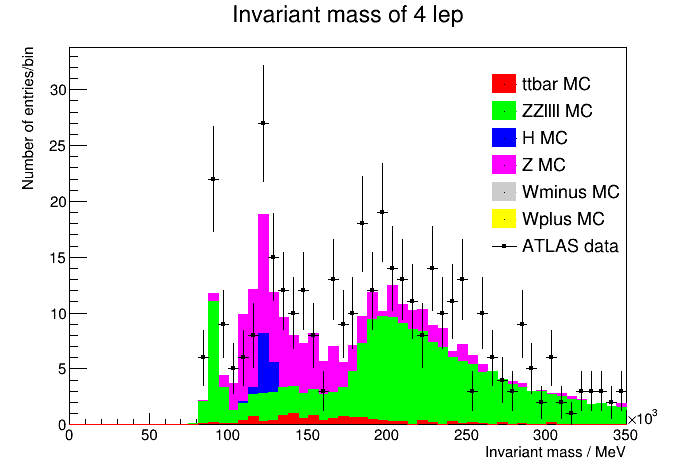
\includegraphics[width=0.85\linewidth]{plots/02-03-2021/18-00.png}
    \caption{Invariant mass plot using ATLAS and Higgs MC data.  Cuts: lep-n == 4, only allowed end products: == e+e- mu+mu-, e+e-e+e-, mu+mu- mu+mu-, with one lepton pair with invariant mass of $60 GeV < m_{ll} < 150 GeV$ and the other $m_{ll} < 150 GeV$}
    \label{fig:18:00_02-03-21}
\end{figure}
%%%%%%%%%%%%%%%%%%%%%%%%%%%%%%%%%%%%%%%%%%%%%%%%%%%%%%%%%%%%%%%%%%%%%%%%%%%%%%%%%%%%%%%%%%%%%%%%%%%%%%%%%%%%%%%%%%%%%%%%
\begin{figure}[h!]
    \centering
    \begin{minipage}{0.5\textwidth}
        \centering
        \includegraphics[width=\linewidth]{plots/02-03-2021/}
        (A)
    \end{minipage}\hfill
    \begin{minipage}{0.5\textwidth}
        \centering
        \includegraphics[width=\linewidth]{plots/02-03-2021/}
        (B)
    \end{minipage}
    \caption{(A)  (B)}
    \label{}
\end{figure}
